% !TeX root = RJwrapper.tex
\title{Toronto Airbnb data research. Application of Supervised Learning Methods
and Unsupervised Learning Methods}
\author{by Ketao Li, Kush Halani, Josue Romain, Juan Peña}

\maketitle

\abstract{%
From thousands of listings in different cities, Airbnb has become a
massive sink of information. Data provided by homeowners are often big,
messy, yet, extremely useful. The goal of this project is to extract
knowledge from these datasets by applying techniques and methodologies
common in data mining.As more homeowners put their properties on the
platform, Airbnb is able to suggest appropriate prices for the listings
based on machine learning models trained over large sets of data. Our
team aims to predict the prices of the listings in Toronto, to allow
homeowners to price their properties appropriately. Specifically, we
seek to answer the following question: What prices should Airbnb suggest
to their hosts given a set of features about the listing? This question
is important because as more data becomes available, more intelligence
can be extracted using modern machine learning tools. Therefore, it is
worthwhile in exploring data driven analyses similar to those presented
in this report as they are likely to improve experience for both hosts
and customers, and ultimately add value to the company.Our team also try
to cluster the listings in groups.
}

\hypertarget{business-understanding}{%
\subsection{1. Business Understanding}\label{business-understanding}}

\hypertarget{determine-business-objectives}{%
\subsection{1.1 Determine Business
Objectives}\label{determine-business-objectives}}

\hypertarget{background}{%
\subsection{Background}\label{background}}

Airbnb has seen a meteoric growth since its inception in 2008 with the
number of rentals listed on its website growing exponentially each year.
Airbnb has successfully disrupted the traditional hospitality industry
as more and more travellers, not just the ones who are looking for a
bang for their buck but also business travellers resort to Airbnb as
their premier accommodation provider. Toronto has been one of the
hottest markets for Airbnb in Canada, with over 26,000 listings as of
Feb 2020. This means there are over 40 homes being rented out per square
km in Toronto on Airbnb! One can perhaps attribute the success of Airbnb
in Toronto to the high rates charged by the hotels, which are primarily
driven by the exorbitant rental prices in the city.

\hypertarget{businnes-objectives}{%
\subsection{Businnes objectives}\label{businnes-objectives}}

\begin{itemize}
\item
  To stablish how do the location, room type, number of reviews,
  availability, number of reviews, minimum nights and host listing count
  can affect rental rates.
\item
  To establish some groups that can be suggested by Airbnb platform for
  different kind of preferences.
\end{itemize}

\hypertarget{business-success-criteria}{%
\subsection{Business success criteria}\label{business-success-criteria}}

Give useful insights for current property owners or future ones to make
more effective listing

\hypertarget{assess-situation}{%
\subsection{1.2 Assess Situation}\label{assess-situation}}

\hypertarget{inventory-of-resources}{%
\subsection{Inventory of resources}\label{inventory-of-resources}}

Machine learning engineers - Ketao Li, Kush Halani, Josue Romain, Juan
Peña

Public Dataset: license CC0: Public Domain

\begin{itemize}
\tightlist
\item
  Toronto AIRBNB open data. Airbnb listing and metrics.
  \href{http://insideairbnb.com/get-the-data.html}{Airbnb}
\end{itemize}

GitHub site. - \url{https://github.com/K2J2PGROUP9/ML1000-3}

\hypertarget{determine-data-mining-goals}{%
\subsection{1.3. Determine Data Mining
Goals}\label{determine-data-mining-goals}}

\hypertarget{data-minning-goals}{%
\subsection{Data minning goals}\label{data-minning-goals}}

This study pursues two goals. The main objective is to predict the
airbnb rental rate as accurate as possible. We will employ CRISP-DM
methodology (Ref: \cite{mining}) and supervised learning approach, to
achieve this goal.

We are also motivated to cluster the toronto airbnb listings in groups.
The questions we will try to address are:

\begin{itemize}
\tightlist
\item
  If there are specific groups of listings that share similar features
\item
  If yes, how to use these group information for business.
\end{itemize}

To achieve the second goal we will use unsupervised learning approach.

\hypertarget{data-mining-success-criteria}{%
\subsection{Data mining success
criteria}\label{data-mining-success-criteria}}

The success criteria of the model is to select the better accuracy based
in the median residual error.

\hypertarget{project-plan}{%
\subsection{Project plan}\label{project-plan}}

\begin{figure}
\centering
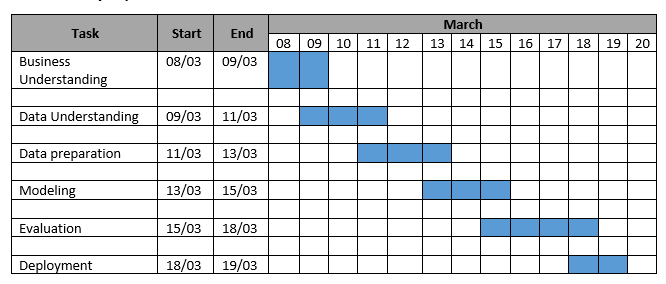
\includegraphics{Project Plan.PNG}
\caption{PROJECT PLAN}
\end{figure}

\hypertarget{apply-the-ethical-ml-framework}{%
\section{Apply the Ethical ML
framework}\label{apply-the-ethical-ml-framework}}

\hypertarget{in-the-problem-definition-and-scope-step}{%
\subsection{In the Problem definition and scope
step}\label{in-the-problem-definition-and-scope-step}}

In the problem identification, we all agree in the group 9 that we want
to develop a tool that help Airbnb's hosts to establish a rental price
for a place as accurate as possible, also to cluster the existing
listings based in similar features. we will be using several models of
prediction and clustering.

Although individuals could be identified by its places, those are not
negatively impacted, there is not any personal identification and we
will not use aggregate information from another sources.

We can see that There could be a risk to individualize each person in
the dataset if someone can access to another dataset that relate the the
Host ID, the Hostname with the PII.

\hypertarget{in-the-design-step}{%
\subsection{In the Design step}\label{in-the-design-step}}

To ensure we all interpreted the outputs of the model we clarify that we
will find through the machine learning model selected, a sugested price
for a place to rent in Toronto's Airbnb platform based in some features.

\hypertarget{in-the-data-collection-and-retention-step}{%
\subsection{In the data collection and retention
step}\label{in-the-data-collection-and-retention-step}}

We just use data from the dataset AB\_TOR\_2019.

In the dataset there is no any underrepresented group because is a full
data about hosts in Toronto, but could be some kind of bias about
locations where people from some countries use to live.

\hypertarget{in-data-processing-step}{%
\subsection{In data processing step}\label{in-data-processing-step}}

Although there is information in the data set that can be used for a
proxy ethnic backgrounnd, the risk is low and could be helpfull for
people looking for a place that match with own ethnicity.

We can identify a risk because we have some columns that could be used
to re-identification, Host ID, Name and the location columns. The host
id and name could be deleted to de-identify the data.

\hypertarget{in-the-model-prototyping-and-qa-testing-step}{%
\subsection{In the model prototyping and QA testing
step}\label{in-the-model-prototyping-and-qa-testing-step}}

The case we are working on, as is predicting prices for host services,
is no so sensitive but the algorithms we are using for regression and
clustering could be interpretable.

In order to make the model fairer and more accuracy, it is important to
take care with the outliers in the prices so the model would be better
adjusted.

\hypertarget{in-the-deployment-monitoring-and-maintenance}{%
\subsection{In the Deployment, Monitoring and
Maintenance}\label{in-the-deployment-monitoring-and-maintenance}}

When using the model it is good to monitor the performance of it when
update the dataset to take into account possible business model changes
like taxes policies that could originate that the predictions could be
wrong.

\hypertarget{data-understanding}{%
\subsection{2 Data Understanding}\label{data-understanding}}

\hypertarget{collect-initial-data}{%
\subsection{2.1 Collect initial data}\label{collect-initial-data}}

\hypertarget{initial-data-collection-report}{%
\section{Initial data collection
report}\label{initial-data-collection-report}}

This research employs the data set sourced from
\href{http://insideairbnb.com/get-the-data.html}{Airbnb}. This real-life
data comprises 26000 observations of the listing information of Toronto
on Feb 14,2020 with 16 features.

\hypertarget{describe-data}{%
\subsection{2.2 Describe data}\label{describe-data}}

\hypertarget{data-description-report}{%
\subsection{Data description report}\label{data-description-report}}

\begin{longtable}[]{@{}ll@{}}
\toprule
Column Name & Column Description\tabularnewline
\midrule
\endhead
id & listing ID\tabularnewline
name & Listing Title\tabularnewline
host\_id & ID of Host\tabularnewline
host\_name & Name of Host\tabularnewline
neighbourhood\_group & Borough that contains listing\tabularnewline
neighbourhood & Name of neighbourhood that listing is in\tabularnewline
latitude & latitude coordinates of listing\tabularnewline
longitude & longitude coordinates of listing\tabularnewline
room\_type & Type of public space that is being offered\tabularnewline
price & price per night in dollars\tabularnewline
minimum\_nights & minimum number of nights required to book
listing\tabularnewline
number\_of\_reviews & total number of reviews that listing has
accumulated\tabularnewline
last\_review & date in which listing was last reviewed\tabularnewline
reviews\_per\_month & total number of reviews per month\tabularnewline
calculated\_host\_listings\_count & amount of listing per
host\tabularnewline
availability\_365 & number of days per year the listing is
active\tabularnewline
\bottomrule
\end{longtable}

\hypertarget{data-exploration}{%
\subsection{2.3 Data Exploration}\label{data-exploration}}

\hypertarget{data-exploration-report}{%
\subsection{Data exploration report}\label{data-exploration-report}}

\hypertarget{statistics}{%
\subsubsection{Statistics}\label{statistics}}

Firstly we are going to load and examine content and statistics of the
data set

\begin{Schunk}
\begin{Sinput}
data = read.csv("../data/AB_TOR_2019.csv", header = T, 
                na.strings = c("NA","","#NA"),sep=",")
\end{Sinput}
\end{Schunk}

\begin{longtable}[]{@{}lllll@{}}
\caption{\label{tab:dataset_summary1} Toronto Airbnb Dataset
Summary}\tabularnewline
\toprule
\begin{minipage}[b]{0.04\columnwidth}\raggedright
No\strut
\end{minipage} & \begin{minipage}[b]{0.26\columnwidth}\raggedright
Variable\strut
\end{minipage} & \begin{minipage}[b]{0.30\columnwidth}\raggedright
Stats / Values\strut
\end{minipage} & \begin{minipage}[b]{0.18\columnwidth}\raggedright
Freqs (\% of Valid)\strut
\end{minipage} & \begin{minipage}[b]{0.08\columnwidth}\raggedright
Missing\strut
\end{minipage}\tabularnewline
\midrule
\endfirsthead
\toprule
\begin{minipage}[b]{0.04\columnwidth}\raggedright
No\strut
\end{minipage} & \begin{minipage}[b]{0.26\columnwidth}\raggedright
Variable\strut
\end{minipage} & \begin{minipage}[b]{0.30\columnwidth}\raggedright
Stats / Values\strut
\end{minipage} & \begin{minipage}[b]{0.18\columnwidth}\raggedright
Freqs (\% of Valid)\strut
\end{minipage} & \begin{minipage}[b]{0.08\columnwidth}\raggedright
Missing\strut
\end{minipage}\tabularnewline
\midrule
\endhead
\begin{minipage}[t]{0.04\columnwidth}\raggedright
1\strut
\end{minipage} & \begin{minipage}[t]{0.26\columnwidth}\raggedright
id\\
{[}integer{]}\strut
\end{minipage} & \begin{minipage}[t]{0.30\columnwidth}\raggedright
Mean (sd) : 25700180.4 (11858759.3)\\
min \textless{} med \textless{} max:\\
1419 \textless{} 27306796 \textless{} 42289607\\
IQR (CV) : 19949214.8 (0.5)\strut
\end{minipage} & \begin{minipage}[t]{0.18\columnwidth}\raggedright
23398 distinct values\strut
\end{minipage} & \begin{minipage}[t]{0.08\columnwidth}\raggedright
0\\
(0\%)\strut
\end{minipage}\tabularnewline
\begin{minipage}[t]{0.04\columnwidth}\raggedright
2\strut
\end{minipage} & \begin{minipage}[t]{0.26\columnwidth}\raggedright
name\\
{[}factor{]}\strut
\end{minipage} & \begin{minipage}[t]{0.30\columnwidth}\raggedright
1. '' BEAUTIFULLY RENOVATE\\
2. `NEW' Downtown Toronto 4\\
3. `Treasure Box' Studio Apa\\
{[} 22920 others {]}\strut
\end{minipage} & \begin{minipage}[t]{0.18\columnwidth}\raggedright
1 ( 0.0\%)\\
1 ( 0.0\%)\\
1 ( 0.0\%)\\
23394 (100.0\%)\strut
\end{minipage} & \begin{minipage}[t]{0.08\columnwidth}\raggedright
1\\
(0\%)\strut
\end{minipage}\tabularnewline
\begin{minipage}[t]{0.04\columnwidth}\raggedright
3\strut
\end{minipage} & \begin{minipage}[t]{0.26\columnwidth}\raggedright
host\_id\\
{[}integer{]}\strut
\end{minipage} & \begin{minipage}[t]{0.30\columnwidth}\raggedright
Mean (sd) : 104673805.4 (98549416.1)\\
min \textless{} med \textless{} max:\\
1565 \textless{} 67279440 \textless{} 335942960\\
IQR (CV) : 158597247 (0.9)\strut
\end{minipage} & \begin{minipage}[t]{0.18\columnwidth}\raggedright
15031 distinct values\strut
\end{minipage} & \begin{minipage}[t]{0.08\columnwidth}\raggedright
0\\
(0\%)\strut
\end{minipage}\tabularnewline
\begin{minipage}[t]{0.04\columnwidth}\raggedright
4\strut
\end{minipage} & \begin{minipage}[t]{0.26\columnwidth}\raggedright
host\_name\\
{[}factor{]}\strut
\end{minipage} & \begin{minipage}[t]{0.30\columnwidth}\raggedright
1. (Email hidden by Airbnb)\\
2. (Phone number hidden by A\\
3. (Wendy) Uyen\\
{[} 6243 others {]}\strut
\end{minipage} & \begin{minipage}[t]{0.18\columnwidth}\raggedright
1 ( 0.0\%)\\
1 ( 0.0\%)\\
1 ( 0.0\%)\\
23392 (100.0\%)\strut
\end{minipage} & \begin{minipage}[t]{0.08\columnwidth}\raggedright
3\\
(0.01\%)\strut
\end{minipage}\tabularnewline
\begin{minipage}[t]{0.04\columnwidth}\raggedright
5\strut
\end{minipage} & \begin{minipage}[t]{0.26\columnwidth}\raggedright
neighbourhood\_group\\
{[}logical{]}\strut
\end{minipage} & \begin{minipage}[t]{0.30\columnwidth}\raggedright
All NA's\strut
\end{minipage} & \begin{minipage}[t]{0.18\columnwidth}\raggedright
\strut
\end{minipage} & \begin{minipage}[t]{0.08\columnwidth}\raggedright
23398\\
(100\%)\strut
\end{minipage}\tabularnewline
\begin{minipage}[t]{0.04\columnwidth}\raggedright
6\strut
\end{minipage} & \begin{minipage}[t]{0.26\columnwidth}\raggedright
neighbourhood\\
{[}factor{]}\strut
\end{minipage} & \begin{minipage}[t]{0.30\columnwidth}\raggedright
1. Agincourt North\\
2. Agincourt South-Malvern W\\
3. Alderwood\\
{[} 137 others {]}\strut
\end{minipage} & \begin{minipage}[t]{0.18\columnwidth}\raggedright
49 ( 0.2\%)\\
97 ( 0.4\%)\\
37 ( 0.2\%)\\
23215 (99.2\%)\strut
\end{minipage} & \begin{minipage}[t]{0.08\columnwidth}\raggedright
0\\
(0\%)\strut
\end{minipage}\tabularnewline
\begin{minipage}[t]{0.04\columnwidth}\raggedright
7\strut
\end{minipage} & \begin{minipage}[t]{0.26\columnwidth}\raggedright
latitude\\
{[}numeric{]}\strut
\end{minipage} & \begin{minipage}[t]{0.30\columnwidth}\raggedright
Mean (sd) : 43.7 (0)\\
min \textless{} med \textless{} max:\\
43.6 \textless{} 43.7 \textless{} 43.8\\
IQR (CV) : 0.1 (0)\strut
\end{minipage} & \begin{minipage}[t]{0.18\columnwidth}\raggedright
10184 distinct values\strut
\end{minipage} & \begin{minipage}[t]{0.08\columnwidth}\raggedright
0\\
(0\%)\strut
\end{minipage}\tabularnewline
\begin{minipage}[t]{0.04\columnwidth}\raggedright
8\strut
\end{minipage} & \begin{minipage}[t]{0.26\columnwidth}\raggedright
longitude\\
{[}numeric{]}\strut
\end{minipage} & \begin{minipage}[t]{0.30\columnwidth}\raggedright
Mean (sd) : -79.4 (0.1)\\
min \textless{} med \textless{} max:\\
-79.6 \textless{} -79.4 \textless{} -79.1\\
IQR (CV) : 0 (0)\strut
\end{minipage} & \begin{minipage}[t]{0.18\columnwidth}\raggedright
12918 distinct values\strut
\end{minipage} & \begin{minipage}[t]{0.08\columnwidth}\raggedright
0\\
(0\%)\strut
\end{minipage}\tabularnewline
\begin{minipage}[t]{0.04\columnwidth}\raggedright
9\strut
\end{minipage} & \begin{minipage}[t]{0.26\columnwidth}\raggedright
room\_type\\
{[}factor{]}\strut
\end{minipage} & \begin{minipage}[t]{0.30\columnwidth}\raggedright
1. Entire home/apt\\
2. Hotel room\\
3. Private room\\
4. Shared room\strut
\end{minipage} & \begin{minipage}[t]{0.18\columnwidth}\raggedright
14991 (64.1\%)\\
69 ( 0.3\%)\\
7913 (33.8\%)\\
425 ( 1.8\%)\strut
\end{minipage} & \begin{minipage}[t]{0.08\columnwidth}\raggedright
0\\
(0\%)\strut
\end{minipage}\tabularnewline
\begin{minipage}[t]{0.04\columnwidth}\raggedright
10\strut
\end{minipage} & \begin{minipage}[t]{0.26\columnwidth}\raggedright
price\\
{[}integer{]}\strut
\end{minipage} & \begin{minipage}[t]{0.30\columnwidth}\raggedright
Mean (sd) : 147.6 (325.8)\\
min \textless{} med \textless{} max:\\
0 \textless{} 99 \textless{} 13256\\
IQR (CV) : 94 (2.2)\strut
\end{minipage} & \begin{minipage}[t]{0.18\columnwidth}\raggedright
479 distinct values\strut
\end{minipage} & \begin{minipage}[t]{0.08\columnwidth}\raggedright
0\\
(0\%)\strut
\end{minipage}\tabularnewline
\begin{minipage}[t]{0.04\columnwidth}\raggedright
11\strut
\end{minipage} & \begin{minipage}[t]{0.26\columnwidth}\raggedright
minimum\_nights\\
{[}integer{]}\strut
\end{minipage} & \begin{minipage}[t]{0.30\columnwidth}\raggedright
Mean (sd) : 6.8 (28.6)\\
min \textless{} med \textless{} max:\\
1 \textless{} 2 \textless{} 1125\\
IQR (CV) : 2 (4.2)\strut
\end{minipage} & \begin{minipage}[t]{0.18\columnwidth}\raggedright
101 distinct values\strut
\end{minipage} & \begin{minipage}[t]{0.08\columnwidth}\raggedright
0\\
(0\%)\strut
\end{minipage}\tabularnewline
\begin{minipage}[t]{0.04\columnwidth}\raggedright
12\strut
\end{minipage} & \begin{minipage}[t]{0.26\columnwidth}\raggedright
number\_of\_reviews\\
{[}integer{]}\strut
\end{minipage} & \begin{minipage}[t]{0.30\columnwidth}\raggedright
Mean (sd) : 28.5 (52.9)\\
min \textless{} med \textless{} max:\\
0 \textless{} 8 \textless{} 803\\
IQR (CV) : 30 (1.9)\strut
\end{minipage} & \begin{minipage}[t]{0.18\columnwidth}\raggedright
393 distinct values\strut
\end{minipage} & \begin{minipage}[t]{0.08\columnwidth}\raggedright
0\\
(0\%)\strut
\end{minipage}\tabularnewline
\begin{minipage}[t]{0.04\columnwidth}\raggedright
13\strut
\end{minipage} & \begin{minipage}[t]{0.26\columnwidth}\raggedright
last\_review\\
{[}factor{]}\strut
\end{minipage} & \begin{minipage}[t]{0.30\columnwidth}\raggedright
1. 2010-08-11\\
2. 2011-08-30\\
3. 2012-07-16\\
{[} 1419 others {]}\strut
\end{minipage} & \begin{minipage}[t]{0.18\columnwidth}\raggedright
1 ( 0.0\%)\\
1 ( 0.0\%)\\
1 ( 0.0\%)\\
19023 (100.0\%)\strut
\end{minipage} & \begin{minipage}[t]{0.08\columnwidth}\raggedright
4372\\
(18.69\%)\strut
\end{minipage}\tabularnewline
\begin{minipage}[t]{0.04\columnwidth}\raggedright
14\strut
\end{minipage} & \begin{minipage}[t]{0.26\columnwidth}\raggedright
reviews\_per\_month\\
{[}numeric{]}\strut
\end{minipage} & \begin{minipage}[t]{0.30\columnwidth}\raggedright
Mean (sd) : 1.8 (2.1)\\
min \textless{} med \textless{} max:\\
0 \textless{} 1 \textless{} 16.9\\
IQR (CV) : 2.2 (1.2)\strut
\end{minipage} & \begin{minipage}[t]{0.18\columnwidth}\raggedright
1045 distinct values\strut
\end{minipage} & \begin{minipage}[t]{0.08\columnwidth}\raggedright
4372\\
(18.69\%)\strut
\end{minipage}\tabularnewline
\begin{minipage}[t]{0.04\columnwidth}\raggedright
15\strut
\end{minipage} & \begin{minipage}[t]{0.26\columnwidth}\raggedright
calculated\_host\_listings\_count\\
{[}integer{]}\strut
\end{minipage} & \begin{minipage}[t]{0.30\columnwidth}\raggedright
Mean (sd) : 5.3 (12.2)\\
min \textless{} med \textless{} max:\\
1 \textless{} 1 \textless{} 119\\
IQR (CV) : 3 (2.3)\strut
\end{minipage} & \begin{minipage}[t]{0.18\columnwidth}\raggedright
43 distinct values\strut
\end{minipage} & \begin{minipage}[t]{0.08\columnwidth}\raggedright
0\\
(0\%)\strut
\end{minipage}\tabularnewline
\begin{minipage}[t]{0.04\columnwidth}\raggedright
16\strut
\end{minipage} & \begin{minipage}[t]{0.26\columnwidth}\raggedright
availability\_365\\
{[}integer{]}\strut
\end{minipage} & \begin{minipage}[t]{0.30\columnwidth}\raggedright
Mean (sd) : 126.2 (127.3)\\
min \textless{} med \textless{} max:\\
0 \textless{} 85 \textless{} 365\\
IQR (CV) : 225 (1)\strut
\end{minipage} & \begin{minipage}[t]{0.18\columnwidth}\raggedright
366 distinct values\strut
\end{minipage} & \begin{minipage}[t]{0.08\columnwidth}\raggedright
0\\
(0\%)\strut
\end{minipage}\tabularnewline
\bottomrule
\end{longtable}

\begin{Schunk}
\begin{Sinput}
#head(data)
#summary(data)
#str(data)
\end{Sinput}
\end{Schunk}

Table \ref{tab:dataset_summary} describes main statistical parameters of
each column. Here is a look at the data sample.

\% latex table generated in R 3.6.3 by xtable 1.8-4 package \% Wed Mar
18 20:50:17 2020

\begin{table}[ht]
\centering
\scalebox{0.6}{
\begin{tabular}{rlrlllrr}
  \hline
id & name & host\_id & host\_name & neighbourhood\_group & neighbourhood & latitude & longitude \\ 
  \hline
1419 & Beautiful home in amazing area! & 1565 & Alexandra &  & Little Portugal & 43.65 & -79.42 \\ 
  8077 & Downtown Harbourfront Private Room & 22795 & Kathie \& Larry &  & Waterfront Communities-The Island & 43.64 & -79.38 \\ 
  12604 & Seaton Village Parlour Bedroom & 48239 & Rona &  & Annex & 43.67 & -79.42 \\ 
  23691 & Queen Bedroom close to downtown & 93825 & Yohan \& Sarah &  & Briar Hill-Belgravia & 43.70 & -79.45 \\ 
  26654 & World Class downtown @CN Tower Theatre MTCC games! & 113345 & Adela &  & Waterfront Communities-The Island & 43.65 & -79.39 \\ 
  27423 & Executive Studio Unit- Ideal for One Person & 118124 & Brent &  & Greenwood-Coxwell & 43.67 & -79.33 \\ 
  30931 & Downtown Toronto - Waterview Condo & 22795 & Kathie \& Larry &  & Waterfront Communities-The Island & 43.64 & -79.38 \\ 
  40456 & Downtown 2  Bdr.Apt with King Size Bed and Parking & 174063 & Denis &  & South Parkdale & 43.64 & -79.44 \\ 
  41887 & Great location & 183071 & Kyle &  & Oakridge & 43.69 & -79.29 \\ 
  43964 & Bright entire 2-bedrm basement suite private entry & 192364 & Mitra &  & Wexford/Maryvale & 43.75 & -79.29 \\ 
  44452 & Yonge \& Bloor Studio Skyline & 195095 & Urbano &  & Rosedale-Moore Park & 43.67 & -79.39 \\ 
  45399 & Fountain View Studio - Eaton center & 195095 & Urbano &  & Church-Yonge Corridor & 43.66 & -79.38 \\ 
   \hline
\end{tabular}
}
\end{table}

\% latex table generated in R 3.6.3 by xtable 1.8-4 package \% Wed Mar
18 20:50:17 2020

\begin{table}[ht]
\centering
\scalebox{0.6}{
\begin{tabular}{lrrrlrrr}
  \hline
room\_type & price & minimum\_nights & number\_of\_reviews & last\_review & reviews\_per\_month & calculated\_host\_listings\_count & availability\_365 \\ 
  \hline
Entire home/apt & 469 &   4 &   7 & 2017-12-04 & 0.13 &   1 &   0 \\ 
  Private room &  99 & 180 & 169 & 2013-08-27 & 1.32 &   2 &   0 \\ 
  Private room &  66 &   1 &   0 &  &  &   1 &   0 \\ 
  Private room &  72 &   1 & 217 & 2019-12-22 & 1.84 &   2 &   0 \\ 
  Entire home/apt & 199 &   4 &  39 & 2020-01-06 & 0.35 &   5 & 365 \\ 
  Entire home/apt &  54 & 120 &  26 & 2011-08-30 & 0.22 &   1 &   0 \\ 
  Entire home/apt & 133 & 180 &   1 & 2010-08-11 & 0.01 &   2 & 365 \\ 
  Entire home/apt &  99 &  30 & 109 & 2019-11-08 & 0.94 &   5 & 250 \\ 
  Entire home/apt &  69 &   2 &  82 & 2019-09-02 & 2.09 &   2 & 270 \\ 
  Entire home/apt &  90 &   2 &  30 & 2019-08-05 & 0.79 &   1 & 365 \\ 
  Entire home/apt & 121 &   1 &  50 & 2019-12-24 & 0.44 &  13 & 363 \\ 
  Entire home/apt & 121 &   1 &  78 & 2019-11-07 & 0.69 &  13 & 363 \\ 
   \hline
\end{tabular}
}
\caption{\label{tab:dataset_head} Toronto Airbnb Data Sample} 
\end{table}

\hypertarget{verify-data-quality}{%
\subsection{2.4 Verify data quality}\label{verify-data-quality}}

\hypertarget{data-quality-report}{%
\subsection{Data quality report}\label{data-quality-report}}

\#\#\#Missing data

\begin{Schunk}
\begin{figure}[H]

{\centering \includegraphics{main_files/figure-latex/plot_notes2-1} 

}

\caption[Missing data]{Missing data}\label{fig:plot_notes2}
\end{figure}
\end{Schunk}

\begin{Schunk}
\begin{Sinput}
summary(a)
\end{Sinput}
\begin{Soutput}

 Missings per variable: 
                       Variable Count
                             id     0
                           name     1
                        host_id     0
                      host_name     3
            neighbourhood_group 23398
                  neighbourhood     0
                       latitude     0
                      longitude     0
                      room_type     0
                          price     0
                 minimum_nights     0
              number_of_reviews     0
                    last_review  4372
              reviews_per_month  4372
 calculated_host_listings_count     0
               availability_365     0

 Missings in combinations of variables: 
                    Combinations Count      Percent
 0:0:0:0:1:0:0:0:0:0:0:0:0:0:0:0 19023 81.301820668
 0:0:0:0:1:0:0:0:0:0:0:0:1:1:0:0  4371 18.681083853
 0:0:0:1:1:0:0:0:0:0:0:0:0:0:0:0     2  0.008547739
 0:0:0:1:1:0:0:0:0:0:0:0:1:1:0:0     1  0.004273870
 0:1:0:0:1:0:0:0:0:0:0:0:0:0:0:0     1  0.004273870
\end{Soutput}
\end{Schunk}

There are some missing data for neighbourhood\_group,last\_review and
reviews\_per\_month.It's very strange that most of the
neighbourhood\_group miss in Toronto.We decide to ignore this feature.

\hypertarget{data-transformation}{%
\subsubsection{Data Transformation}\label{data-transformation}}

\hypertarget{data-preparation}{%
\subsection{3. Data preparation}\label{data-preparation}}

We need do some some data transformation.

\begin{Schunk}
\begin{Sinput}
customerData <- data %>% 
  mutate( last_review= as.Date(last_review)) 
         
customerData <- customerData %>% 
  mutate( last_review= as.numeric(as.Date("2020-02-15")-last_review)) 

customerData <- customerData %>% 
  mutate( room_type= as.numeric(room_type) )

#customerData <- customerData %>% 
#  mutate(last_review = as.numeric(as.Date("2020-02-15")-last_review))

#glimpse(customerData)
\end{Sinput}
\end{Schunk}

We drop neighbourhood\_group and other missing data.

\begin{Schunk}
\begin{Sinput}
customerData1 = subset(customerData,select = -neighbourhood_group)
customerData1 = customerData1 %>%filter(complete.cases(.)) 
glimpse(customerData1)
\end{Sinput}
\begin{Soutput}
Observations: 19,023
Variables: 15
$ id                             <int> 1419, 8077, 23691, 26654, 27423, 309...
$ name                           <fct> "Beautiful home in amazing area!", "...
$ host_id                        <int> 1565, 22795, 93825, 113345, 118124, ...
$ host_name                      <fct> Alexandra, Kathie & Larry, Yohan & S...
$ neighbourhood                  <fct> Little Portugal, Waterfront Communit...
$ latitude                       <dbl> 43.64617, 43.64105, 43.69602, 43.645...
$ longitude                      <dbl> -79.42451, -79.37628, -79.45468, -79...
$ room_type                      <dbl> 1, 3, 3, 1, 1, 1, 1, 1, 1, 1, 1, 3, ...
$ price                          <int> 469, 99, 72, 199, 54, 133, 99, 69, 9...
$ minimum_nights                 <int> 4, 180, 1, 4, 120, 180, 30, 2, 2, 1,...
$ number_of_reviews              <int> 7, 169, 217, 39, 26, 1, 109, 82, 30,...
$ last_review                    <dbl> 803, 2363, 55, 40, 3091, 3475, 99, 1...
$ reviews_per_month              <dbl> 0.13, 1.32, 1.84, 0.35, 0.22, 0.01, ...
$ calculated_host_listings_count <int> 1, 2, 2, 5, 1, 2, 5, 2, 1, 13, 13, 1...
$ availability_365               <int> 0, 0, 0, 365, 0, 365, 250, 270, 365,...
\end{Soutput}
\begin{Sinput}
#b = aggr(customerData1)
#plot(b)
\end{Sinput}
\end{Schunk}

\#\#\#data visualization

\begin{Schunk}
\begin{Sinput}
# histogram with added parameters
hist(customerData1$number_of_reviews,
main="number_of_reviews",
xlab="number_of_reviews",
breaks=10000,
xlim=c(0,300),
col="darkmagenta",
freq=FALSE
)
\end{Sinput}


\begin{center}\includegraphics{main_files/figure-latex/unnamed-chunk-7-1} \end{center}

\end{Schunk}

\begin{Schunk}
\begin{Sinput}
# histogram with added parameters
hist(customerData1$last_review,
main="last_review",
xlab="last_review",
breaks=10000,
xlim=c(0,300),
col="darkmagenta",
freq=FALSE
)
\end{Sinput}


\begin{center}\includegraphics{main_files/figure-latex/unnamed-chunk-8-1} \end{center}

\end{Schunk}

\begin{Schunk}
\begin{Sinput}
# histogram with added parameters
hist(customerData1$availability_365,
main="availability_365",
xlab="availability_365",
breaks=10000,
xlim=c(0,300),
col="darkmagenta",
freq=FALSE
)
\end{Sinput}


\begin{center}\includegraphics{main_files/figure-latex/unnamed-chunk-9-1} \end{center}

\end{Schunk}

Hosts on Airbnb offer a wide variety of spaces, ranging from shared
rooms to private islands.

All homes are grouped into the following three room types:

Entire place Private room Shared room hotel room

Entire place Entire places are best if you're seeking a home away from
home. With an entire place, you'll have the whole space to yourself.
This usually includes a bedroom, a bathroom, a kitchen, and a separate,
dedicated entrance. Hosts should note in the description if they'll be
on the property or not (e.g.: ``Host occupies first floor of the
home''), and provide further details on the listing.

Private rooms Private rooms are great for when you prefer a little
privacy, and still value a local connection. When you book a private
room, you'll have your own private room for sleeping and may share some
spaces with others. You might need to walk through indoor spaces that
another host or guest may occupy to get to your room.

Shared rooms Shared rooms are for when you don't mind sharing a space
with others. When you book a shared room, you'll be sleeping in a space
that is shared with others and share the entire space with other people.
Shared rooms are popular among flexible travellers looking for new
friends and budget-friendly stays.

\begin{Schunk}
\begin{Sinput}
room = customerData1 %>%
  group_by(room_type = factor(room_type, labels = c("Entire home/apt","Hotel room","Private room","Shared room")))  %>%
  summarise(COUNT = n())
p1 = ggplot(room,aes(x=room_type, y = COUNT, fill = room_type)) + 
      geom_bar(stat = "identity", alpha = 0.7) +  theme(axis.text.x=element_blank(),
      axis.ticks.x=element_blank())
plot(p1)
\end{Sinput}


\begin{center}\includegraphics{main_files/figure-latex/unnamed-chunk-10-1} \end{center}

\end{Schunk}

\begin{Schunk}
\begin{Sinput}
mytable <- table(customerData1$room_type)
lbls <-  c("Entire home/apt","Hotel room","Private room","Shared room")
pie(mytable, labels = lbls,col=rainbow(length(lbls)),
   main="Pie Chart of room")
\end{Sinput}


\begin{center}\includegraphics{main_files/figure-latex/unnamed-chunk-11-1} \end{center}

\end{Schunk}

Price The most important (target) variable is price.

\begin{Schunk}
\begin{Sinput}
ggplot(customerData1, aes(price)) +
  geom_histogram(bins = 30, aes(y = ..density..), fill = "purple") + 
  geom_density(alpha = 0.2, fill = "purple") +
  th +
  ggtitle("Distribution of price",
          subtitle = "The distribution is very skewed") +
  theme(axis.title = element_text(), axis.title.x = element_text()) +
  geom_vline(xintercept = round(mean(customerData1$price), 2), size = 2, linetype = 3)
\end{Sinput}


\begin{center}\includegraphics{main_files/figure-latex/unnamed-chunk-12-1} \end{center}

\end{Schunk}

Histogram \& Density with log10 transformation Since the original
distribution is very skewed, logarithmic transformation can be used to
gain better insight into data.

\begin{Schunk}
\begin{Sinput}
ggplot(customerData1, aes(price)) +
  geom_histogram(bins = 30, aes(y = ..density..), fill = "purple") + 
  geom_density(alpha = 0.2, fill = "purple") +
  th +
  ggtitle("Transformed distribution of price",
          subtitle = expression("With" ~'log'[10] ~ "transformation of x-axis")) +
  #theme(axis.title = element_text(), axis.title.x = element_text()) +
  geom_vline(xintercept = round(mean(customerData1$price), 2), size = 2, linetype = 3) +
  scale_x_log10() #+
\end{Sinput}


\begin{center}\includegraphics{main_files/figure-latex/unnamed-chunk-13-1} \end{center}

\begin{Sinput}
  #annotate("text", x = 1800, y = 0.75,label = paste("Mean price = ", paste0(round(mean(customerData1$price), 2), "$")),
  #         color =  "#32CD32", size = 8)
\end{Sinput}
\end{Schunk}

Price \& Availability

\begin{Schunk}
\begin{Sinput}
ggplot(customerData1, aes(availability_365, price)) +
  th +
  geom_point(alpha = 0.2, color = "slateblue") +
  geom_density(stat = "identity", alpha = 0.2) +
  xlab("Availability during year") +
  ylab("Price") +
  ggtitle("Relationship between availability",
          subtitle = "there is not clear relationship") 
\end{Sinput}


\begin{center}\includegraphics{main_files/figure-latex/unnamed-chunk-14-1} \end{center}

\end{Schunk}

It's hard to see clear pattern, but there's a lot of expensive objects
with few available days and many available days.

Price \& Number Of Reviews

\begin{Schunk}
\begin{Sinput}
ggplot(customerData1, aes(number_of_reviews, price)) +
  th + theme(axis.title = element_text(), axis.title.x = element_text()) +
  geom_point(aes(size = price), alpha = 0.05, color = "slateblue") +
  xlab("Number of reviews") +
  ylab("Price") +
  ggtitle("Relationship between number of reviews",
          subtitle = "The most expensive objects have small number of reviews (or 0)")
\end{Sinput}


\begin{center}\includegraphics{main_files/figure-latex/unnamed-chunk-15-1} \end{center}

\end{Schunk}

\begin{Schunk}
\begin{Sinput}
df  <- customerData1  %>% select("price","number_of_reviews","minimum_nights")
cor(df)
\end{Sinput}
\begin{Soutput}
                         price number_of_reviews minimum_nights
price              1.000000000      -0.009435758   -0.003047704
number_of_reviews -0.009435758       1.000000000   -0.043245174
minimum_nights    -0.003047704      -0.043245174    1.000000000
\end{Soutput}
\begin{Sinput}
corrplot(cor(df))
\end{Sinput}


\begin{center}\includegraphics{main_files/figure-latex/unnamed-chunk-16-1} \end{center}

\end{Schunk}

Below is a plot of the top 10 neighborhoods by number of listings.

\begin{Schunk}
\begin{Sinput}
customerData1 %>%
    group_by(neighbourhood) %>%
    summarize(num_listings = n(), 
              borough = unique(neighbourhood)) %>%
    top_n(n = 10, wt = num_listings) %>%
    ggplot(aes(x = fct_reorder(neighbourhood, num_listings), 
               y = num_listings, fill = borough)) +
    geom_col() +
    coord_flip() +
    theme(legend.position = "bottom") +
    labs(title = "Top 10 neighborhoods by no. of listings",
         x = "Neighborhood", y = "No. of listings")
\end{Sinput}


\begin{center}\includegraphics{main_files/figure-latex/unnamed-chunk-17-1} \end{center}

\end{Schunk}

The plot below shows the distribution of price by room type. (Note that
the y-axis is on a log scale.) There is much variation in price within
each room type. Overall, it looks like ``Entire home/apt'' listings are
slightly pricier than ``Private room'', which in turn are more expensive
than ``Shared room''. This makes intuitive sense.

\begin{Schunk}
\begin{Sinput}
ggplot(data, aes(x = room_type, y = price)) +
    geom_violin() +
    scale_y_log10()
\end{Sinput}


\begin{center}\includegraphics{main_files/figure-latex/unnamed-chunk-18-1} \end{center}

\end{Schunk}

Map of the top 20 most expensive listings

\begin{Schunk}
\begin{Sinput}
# get top 20 listings by price
top_df <- customerData1 %>% top_n(n = 20, wt = price)

# get background map
top_height <- max(top_df$latitude) - min(top_df$latitude)
top_width <- max(top_df$longitude) - min(top_df$longitude)
top_borders <- c(bottom  = min(top_df$latitude)  - 0.1 * top_height,
                 top     = max(top_df$latitude)  + 0.1 * top_height,
                 left    = min(top_df$longitude) - 0.1 * top_width,
                 right   = max(top_df$longitude) + 0.1 * top_width)

top_map <- get_stamenmap(top_borders, zoom = 12, maptype = "toner-lite")

# map of top 50 most expensive
ggmap(top_map) +
    geom_point(data = top_df, mapping = aes(x = longitude, y = latitude,
                                        col = price)) +
    scale_color_gradient(low = "blue", high = "red")
\end{Sinput}


\begin{center}\includegraphics{main_files/figure-latex/unnamed-chunk-19-1} \end{center}

\end{Schunk}

Median price by neighborhood In the map below, each dot is one
neighborhood. The size of the dot depends on the number of listings and
the color of the dot depends on the median price in that neighborhood.

\begin{Schunk}
\begin{Sinput}
nhd_df <- customerData1 %>%
    group_by(neighbourhood) %>%
    summarize(num_listings = n(),
              median_price = median(price),
              long = median(longitude),
              lat = median(latitude),
              borough = unique(neighbourhood))
# map of all listings: one point per neighborhood
height <- max(customerData1$latitude) - min(customerData1$latitude)
width <- max(customerData1$longitude) - min(customerData1$longitude)
borders <- c(bottom  = min(customerData1$latitude)  - 0.1 * height,
             top     = max(customerData1$latitude)  + 0.1 * height,
             left    = min(customerData1$longitude) - 0.1 * width,
             right   = max(customerData1$longitude) + 0.1 * width)

map <- get_stamenmap(borders, zoom = 11, maptype = "toner-lite")
ggmap(map) +
    geom_point(data = nhd_df, mapping = aes(x = long, y = lat,
                                            col = median_price, size = num_listings)) +
    scale_color_gradient(low = "blue", high = "red")
\end{Sinput}


\begin{center}\includegraphics{main_files/figure-latex/unnamed-chunk-20-1} \end{center}

\end{Schunk}

\hypertarget{descriptive-features.}{%
\subsubsection{Descriptive Features.}\label{descriptive-features.}}

\emph{name } is free-text features that might provide additional
insights about the listing. We are going to take a close look at this
feature and decide if we could utilize it.

Lets' begin with the \emph{name}

\begin{Schunk}
\begin{figure}[H]

{\centering \includegraphics{main_files/figure-latex/plot_notes-1} 

}

\caption[Most Common Words in Description]{Most Common Words in Description}\label{fig:plot_notes}
\end{figure}
\end{Schunk}

From the word cloud, we can get some highly frequently used words such
as downtown,bedroom,room,condo,private,apartment.

Unfortunately \emph{name} feature does not provide more knowledge to
what the others features already supply. Thus it will be dropped.

\hypertarget{modeling}{%
\subsection{4. Modeling}\label{modeling}}

\hypertarget{select-modeling-technique}{%
\subsection{4.1 Select Modeling
Technique}\label{select-modeling-technique}}

\hypertarget{modeling-technique}{%
\subsection{Modeling Technique}\label{modeling-technique}}

As this is a price prediction problem, we are going to use Linear
Regresion Model.

\hypertarget{modeling-assumption}{%
\subsection{Modeling assumption}\label{modeling-assumption}}

The asumptions that the model has are:

\begin{itemize}
\tightlist
\item
  Variables are normally ditributed or transformed into it.
\item
  No or little multicolinearity.
\item
  No Auto-correlation.
\item
  No homoscedasticty.
\end{itemize}

\hypertarget{generate-test-design}{%
\subsection{4.2 Generate test design}\label{generate-test-design}}

\hypertarget{test-design}{%
\subsection{Test design}\label{test-design}}

For training purposes we are going to take 70\% of the data and left the
30\% for testing.

\begin{Schunk}
\begin{Sinput}
airbnb_train <- customerData1 %>% sample_frac(.7) %>% filter(price > 0)
airbnb_test  <- anti_join(customerData1, airbnb_train, by = 'id') %>% filter(price > 0)
\end{Sinput}
\end{Schunk}

\hypertarget{build-the-model}{%
\subsection{4.3 Build the model}\label{build-the-model}}

\#\#1st Linear Regression model

\begin{Schunk}
\begin{Sinput}
first_model <- train(price ~ latitude + longitude + room_type + minimum_nights  + availability_365 , data = airbnb_train, method = "lm")
summary(first_model)
\end{Sinput}
\begin{Soutput}

Call:
lm(formula = .outcome ~ ., data = dat)

Residuals:
   Min     1Q Median     3Q    Max 
-196.5  -59.2  -22.3   16.3 9879.3 

Coefficients:
                   Estimate Std. Error t value Pr(>|t|)    
(Intercept)       3.028e+04  3.232e+03   9.369  < 2e-16 ***
latitude         -4.218e+02  3.960e+01 -10.652  < 2e-16 ***
longitude         1.468e+02  2.862e+01   5.129 2.95e-07 ***
room_type        -4.584e+01  1.855e+00 -24.711  < 2e-16 ***
minimum_nights   -9.998e-02  6.689e-02  -1.495    0.135    
availability_365  1.290e-01  1.358e-02   9.504  < 2e-16 ***
---
Signif. codes:  0 '***' 0.001 '**' 0.01 '*' 0.05 '.' 0.1 ' ' 1

Residual standard error: 195.4 on 13307 degrees of freedom
Multiple R-squared:  0.07377,   Adjusted R-squared:  0.07342 
F-statistic:   212 on 5 and 13307 DF,  p-value: < 2.2e-16
\end{Soutput}
\end{Schunk}

\hypertarget{assess-model}{%
\subsection{4.4 Assess Model}\label{assess-model}}

\hypertarget{model-assessment}{%
\subsection{Model assessment}\label{model-assessment}}

This model is not so good. Median residual error is -22.9, while it
should be near 0. R2=0.06 is also not so good.

Let's plot the first model.

\begin{Schunk}
\begin{figure}[H]

{\centering \includegraphics[width=1.1\linewidth]{main_files/figure-latex/plot_feature_selection1-1} 

}

\caption[Number of Predictors vs Accuracy]{Number of Predictors vs Accuracy}\label{fig:plot_feature_selection11}
\end{figure}
\begin{figure}[H]

{\centering \includegraphics[width=1.1\linewidth]{main_files/figure-latex/plot_feature_selection1-2} 

}

\caption[Number of Predictors vs Accuracy]{Number of Predictors vs Accuracy}\label{fig:plot_feature_selection12}
\end{figure}
\begin{figure}[H]

{\centering \includegraphics[width=1.1\linewidth]{main_files/figure-latex/plot_feature_selection1-3} 

}

\caption[Number of Predictors vs Accuracy]{Number of Predictors vs Accuracy}\label{fig:plot_feature_selection13}
\end{figure}
\begin{figure}[H]

{\centering \includegraphics[width=1.1\linewidth]{main_files/figure-latex/plot_feature_selection1-4} 

}

\caption[Number of Predictors vs Accuracy]{Number of Predictors vs Accuracy}\label{fig:plot_feature_selection14}
\end{figure}
\end{Schunk}

\hypertarget{build-the-model-1}{%
\subsection{4.3 Build the model}\label{build-the-model-1}}

\#\#2nd Linear Regression model

\begin{Schunk}
\begin{Sinput}
learn <- airbnb_train %>% filter(price < quantile(airbnb_train$price, 0.9) & price > quantile(airbnb_train$price, 0.1)) %>% tidyr::drop_na()
second_model <- lm(log(price) ~ room_type + latitude + longitude 
                        + number_of_reviews + availability_365
                       + reviews_per_month + 
                     calculated_host_listings_count + minimum_nights, data = learn)
\end{Sinput}
\end{Schunk}

\hypertarget{model-assessment-1}{%
\subsection{Model assessment}\label{model-assessment-1}}

summary(second\_model)

\hypertarget{evaluation}{%
\subsection{5. Evaluation}\label{evaluation}}

\hypertarget{aproved-model}{%
\subsection{Aproved model}\label{aproved-model}}

This model is an improvement. Median residual error is now -0.014, which
is far better than -22.9 from the first model. R2=0.371 means that this
model explains about 50\% variance of target variable. Obviously we
choose the second model for the prediction.

\begin{Schunk}
\begin{figure}[H]

{\centering \includegraphics[width=1.1\linewidth]{main_files/figure-latex/plot_feature_selection-1} 

}

\caption[Number of Predictors vs Accuracy]{Number of Predictors vs Accuracy}\label{fig:plot_feature_selection1}
\end{figure}
\begin{figure}[H]

{\centering \includegraphics[width=1.1\linewidth]{main_files/figure-latex/plot_feature_selection-2} 

}

\caption[Number of Predictors vs Accuracy]{Number of Predictors vs Accuracy}\label{fig:plot_feature_selection2}
\end{figure}
\begin{figure}[H]

{\centering \includegraphics[width=1.1\linewidth]{main_files/figure-latex/plot_feature_selection-3} 

}

\caption[Number of Predictors vs Accuracy]{Number of Predictors vs Accuracy}\label{fig:plot_feature_selection3}
\end{figure}
\begin{figure}[H]

{\centering \includegraphics[width=1.1\linewidth]{main_files/figure-latex/plot_feature_selection-4} 

}

\caption[Number of Predictors vs Accuracy]{Number of Predictors vs Accuracy}\label{fig:plot_feature_selection4}
\end{figure}
\end{Schunk}

\#\#Predict prices for training set

\begin{Schunk}
\begin{Soutput}
[1] 44.81829
\end{Soutput}
\begin{Soutput}
[1] 0.2648741
\end{Soutput}
\end{Schunk}

\begin{Schunk}


\begin{center}\includegraphics{main_files/figure-latex/unnamed-chunk-25-1} \end{center}

\end{Schunk}

\hypertarget{undertanding-the-listing-employing-unsupervised-learning}{%
\section{Undertanding the listing Employing Unsupervised
Learning}\label{undertanding-the-listing-employing-unsupervised-learning}}

\hypertarget{modeling-1}{%
\subsection{4. Modeling}\label{modeling-1}}

\hypertarget{select-modeling-technique-1}{%
\subsection{4.1 Select Modeling
Technique}\label{select-modeling-technique-1}}

\hypertarget{modeling-technique-1}{%
\subsection{Modeling Technique}\label{modeling-technique-1}}

In this section we will apply various clustering methods to cluster the
listings in several groups. We will use Partitioning clustering and
Hierarchical clustering approaches.

Before we apply clustering models to the dataset we should assess
clustering tendency. In order to do so we will employ \textbf{Hopkins}
statistics.

\hypertarget{hopkins-statistics}{%
\subsection{Hopkins Statistics}\label{hopkins-statistics}}

Hopkins statistic is used to assess the clustering tendency of a dataset
by measuring the probability that a given dataset is generated by a
uniform data distribution.(Ref: \cite{mining}). Let's calculate Hopkins
(\textbf{H}) statistics for customerData1:

The \textbf{H} value close to one indicates very good clustering
tendency. The \textbf{H} value around or greater than 0.5 denotes poor
clustering tendency(Ref: \cite{factoextra}).

\begin{Schunk}
\begin{Sinput}
customerData2 = subset(customerData1,select = -id)
customerData2 = subset(customerData2,select = -name)
customerData2 = subset(customerData2,select = -host_id)
customerData2 = subset(customerData2,select = -host_name)
customerData2 = subset(customerData2,select = -neighbourhood)

customerData2 <- customerData2 %>% 
mutate(
       latitude = scale(latitude),
       longitude = scale(longitude),
       price = scale(price),
       minimum_nights = scale(minimum_nights),
       number_of_reviews = scale(number_of_reviews),
       last_review = scale(last_review),
       reviews_per_month  = scale(reviews_per_month ),
       calculated_host_listings_count = scale(calculated_host_listings_count),
       availability_365 = scale(availability_365)
)
#summary(customerData2)
\end{Sinput}
\end{Schunk}

\begin{Schunk}
\begin{Sinput}
H =  get_clust_tendency(customerData2,n = 100, graph = F, seed = 6709)
print(H[["hopkins_stat"]])
\end{Sinput}
\begin{Soutput}
[1] 0.9809828
\end{Soutput}
\end{Schunk}

Perfect! H value is very close to 1. The dataset is clustrable.

\hypertarget{build-the-model-2}{%
\subsection{4.3 Build the model}\label{build-the-model-2}}

\hypertarget{partitioning-clustering-approach}{%
\subsection{Partitioning Clustering
Approach}\label{partitioning-clustering-approach}}

At first, we use Elbow method to get optimal number of clusters for
k-means clustering:

\begin{Schunk}
\begin{Sinput}
set.seed(123)
# Elbow method
fviz_nbclust(customerData2, kmeans, method = "wss") +
    geom_vline(xintercept = 4, linetype = 2)+
  labs(subtitle = "Elbow method")
\end{Sinput}


\begin{center}\includegraphics{main_files/figure-latex/unnamed-chunk-28-1} \end{center}

\end{Schunk}

It seems that the optimal number of clusters is 4.

Let's use kmeans to cluster the dataset.

\begin{Schunk}
\begin{Sinput}
set.seed(123)
k2 <- kmeans(customerData2, centers = 4, nstart = 25)
#k2
fviz_cluster(k2, data = customerData2)
\end{Sinput}


\begin{center}\includegraphics{main_files/figure-latex/unnamed-chunk-29-1} \end{center}

\end{Schunk}

\begin{Schunk}
\begin{Sinput}
group <- k2$cluster
customerData3 <- cbind(customerData1, group)
#write.csv(customerData3, "../shiny/www/mydata1.csv")
\end{Sinput}
\end{Schunk}

\hypertarget{build-the-model-3}{%
\subsection{4.3 Build the model}\label{build-the-model-3}}

\hypertarget{hierarchical-clustering-approache}{%
\subsection{Hierarchical clustering
approache}\label{hierarchical-clustering-approache}}

\begin{Schunk}
\begin{Sinput}
set.seed(123)
d <- dist(customerData2)
c <- hclust(d, method = 'ward.D2')

plot(c)
\end{Sinput}


\begin{center}\includegraphics{main_files/figure-latex/unnamed-chunk-31-1} \end{center}

\end{Schunk}

\begin{Schunk}
\begin{Sinput}
members <- cutree(c,k = 4)

table(members)
#members
\end{Sinput}
\begin{Soutput}
members
   1    2    3    4 
2572 8164 2579 5708 
\end{Soutput}
\end{Schunk}

\hypertarget{evaluation-1}{%
\subsection{5. Evaluation}\label{evaluation-1}}

\hypertarget{aproved-model-1}{%
\subsection{Aproved model}\label{aproved-model-1}}

We decide to accept the kmeans cluster result. K-means clustering with 4
clusters of sizes group1 = 2649, group2 = 9925, group3 = 2800, group4 =
3649

\begin{Schunk}
\begin{Sinput}
group1 <- customerData3 %>% 
  filter(group == 1)

group2 <- customerData3 %>% 
  filter(group == 2)

group3 <- customerData3 %>% 
  filter(group == 3)

group4 <- customerData3 %>% 
  filter(group == 4)
\end{Sinput}
\end{Schunk}

Let's dig out why the listings are clustered to 4 groups. At first,
let's observe every group's geographic distribution.

\begin{Schunk}
\begin{Sinput}
leaflet(group1 %>% select(longitude,latitude)) %>%
  setView(lng = -79.38, lat = 43.75,zoom = 11) %>%
   addTiles() %>% 
  addMarkers(
  clusterOptions = markerClusterOptions())
\end{Sinput}


\begin{center}\includegraphics{main_files/figure-latex/unnamed-chunk-34-1} \end{center}

\end{Schunk}

\begin{Schunk}
\begin{Sinput}
leaflet(group2 %>% select(longitude,latitude)) %>%
  setView(lng = -79.38, lat = 43.75,zoom = 11) %>%
   addTiles() %>% 
  addMarkers(
  clusterOptions = markerClusterOptions())
\end{Sinput}


\begin{center}\includegraphics{main_files/figure-latex/unnamed-chunk-35-1} \end{center}

\end{Schunk}

\begin{Schunk}
\begin{Sinput}
leaflet(group3 %>% select(longitude,latitude)) %>%
  setView(lng = -79.38, lat = 43.75,zoom = 11) %>%
   addTiles() %>% 
  addMarkers(
  clusterOptions = markerClusterOptions())
\end{Sinput}


\begin{center}\includegraphics{main_files/figure-latex/unnamed-chunk-36-1} \end{center}

\end{Schunk}

\begin{Schunk}
\begin{Sinput}
leaflet(group4 %>% select(longitude,latitude)) %>%
  setView(lng = -79.38, lat = 43.75,zoom = 11) %>%
   addTiles() %>% 
  addMarkers(
  clusterOptions = markerClusterOptions())
\end{Sinput}


\begin{center}\includegraphics{main_files/figure-latex/unnamed-chunk-37-1} \end{center}

\end{Schunk}

From the geographic distribution, we can observe that group4, most of
the listings are far from downtown.

Let's observe every group's price distribution.

\begin{Schunk}
\begin{Sinput}
# histogram with added parameters
hist(group1$price,
main="group1Price",
xlab="group1Price",
breaks=100000,
xlim=c(0,500),
col="darkmagenta",
freq=FALSE
)
\end{Sinput}


\begin{center}\includegraphics{main_files/figure-latex/unnamed-chunk-38-1} \end{center}

\end{Schunk}

\begin{Schunk}
\begin{Sinput}
# histogram with added parameters
hist(group2$price,
main="group2Price",
xlab="group2Price",
breaks=100000,
xlim=c(0,500),
col="darkmagenta",
freq=FALSE
)
\end{Sinput}


\begin{center}\includegraphics{main_files/figure-latex/unnamed-chunk-39-1} \end{center}

\end{Schunk}

\begin{Schunk}
\begin{Sinput}
# histogram with added parameters
hist(group3$price,
main="group3Price",
xlab="group3Price",
breaks=100000,
xlim=c(0,500),
col="darkmagenta",
freq=FALSE
)
\end{Sinput}


\begin{center}\includegraphics{main_files/figure-latex/unnamed-chunk-40-1} \end{center}

\end{Schunk}

\begin{Schunk}
\begin{Sinput}
# histogram with added parameters
hist(group4$price,
main="group4Price",
xlab="group4Price",
breaks=100000,
xlim=c(0,500),
col="darkmagenta",
freq=FALSE
)
\end{Sinput}


\begin{center}\includegraphics{main_files/figure-latex/unnamed-chunk-41-1} \end{center}

\end{Schunk}

Obviously in group4, The vast majority of rental prices are concentrated
below 100\$.

Let's list every group's median price.

\begin{Schunk}
\begin{Sinput}
median(group1$price)
\end{Sinput}
\begin{Soutput}
[1] 99
\end{Soutput}
\begin{Sinput}
median(group2$price)
\end{Sinput}
\begin{Soutput}
[1] 117
\end{Soutput}
\begin{Sinput}
median(group3$price)
\end{Sinput}
\begin{Soutput}
[1] 117
\end{Soutput}
\begin{Sinput}
median(group4$price)
\end{Sinput}
\begin{Soutput}
[1] 54
\end{Soutput}
\end{Schunk}

In group1, the rental price is median. Group4 is the cheapest. Group2 \&
Group3 has the same median price.

We're interested in what's the difference between group2 and group3.
Let's dig it further.

\begin{Schunk}
\begin{Sinput}
# histogram with added parameters
hist(group2$minimum_nights,
main="group2 minimum_nights",
xlab="minimum_nights",
breaks=10000,
xlim=c(0,100),
col="darkmagenta",
freq=FALSE
)
\end{Sinput}


\begin{center}\includegraphics{main_files/figure-latex/unnamed-chunk-43-1} \end{center}

\end{Schunk}

\begin{Schunk}
\begin{Sinput}
# histogram with added parameters
hist(group3$minimum_nights,
main="group3 minimum_nights",
xlab="minimum_nights",
breaks=10000,
xlim=c(0,100),
col="darkmagenta",
freq=FALSE
)
\end{Sinput}


\begin{center}\includegraphics{main_files/figure-latex/unnamed-chunk-44-1} \end{center}

\end{Schunk}

\begin{Schunk}
\begin{Sinput}
# histogram with added parameters
hist(group2$number_of_reviews,
main="group2 number_of_reviews",
xlab="minimum_nights",
breaks=10000,
xlim=c(0,500),
col="darkmagenta",
freq=FALSE
)
\end{Sinput}


\begin{center}\includegraphics{main_files/figure-latex/unnamed-chunk-45-1} \end{center}

\end{Schunk}

\begin{Schunk}
\begin{Sinput}
# histogram with added parameters
hist(group3$number_of_reviews,
main="group3 number_of_reviews",
xlab="number_of_reviews",
breaks=10000,
xlim=c(0,500),
col="darkmagenta",
freq=FALSE
)
\end{Sinput}


\begin{center}\includegraphics{main_files/figure-latex/unnamed-chunk-46-1} \end{center}

\end{Schunk}

It seems that the group3 has more reviews that group2.

\begin{Schunk}
\begin{Sinput}
# histogram with added parameters
hist(group2$last_review,
main="group2 last_review",
xlab="last_review",
breaks=10000,
xlim=c(0,200),
col="darkmagenta",
freq=FALSE
)
\end{Sinput}


\begin{center}\includegraphics{main_files/figure-latex/unnamed-chunk-47-1} \end{center}

\end{Schunk}

\begin{Schunk}
\begin{Sinput}
# histogram with added parameters
hist(group3$last_review,
main="group3 last_review",
xlab="last_review",
breaks=10000,
xlim=c(0,200),
col="darkmagenta",
freq=FALSE
)
\end{Sinput}


\begin{center}\includegraphics{main_files/figure-latex/unnamed-chunk-48-1} \end{center}

\end{Schunk}

\begin{Schunk}
\begin{Sinput}
# histogram with added parameters
hist(group2$availability_365,
main="group2 availability_365",
xlab="last_review",
breaks=10000,
xlim=c(0,200),
col="darkmagenta",
freq=FALSE
)
\end{Sinput}


\begin{center}\includegraphics{main_files/figure-latex/unnamed-chunk-49-1} \end{center}

\end{Schunk}

\begin{Schunk}
\begin{Sinput}
# histogram with added parameters
hist(group3$availability_365,
main="group3 availability_365",
xlab="last_review",
breaks=10000,
xlim=c(0,200),
col="darkmagenta",
freq=FALSE
)
\end{Sinput}


\begin{center}\includegraphics{main_files/figure-latex/unnamed-chunk-50-1} \end{center}

\end{Schunk}

It seems that the group3 has more availability\_365 that group2. Let's
summarize every group's characteristic.

Group1: the rental rate is median.

Group2: the rental rate is high, and the attention is low because there
are less reviews in this group.Since most of listings in this group are
located in downtown,they have Convenient transportation.

Group3: the rental rate is high, and the attention is high because there
are more reviews in this group.Since most of listings in this group are
located in downtown,they have Convenient transportation.

Group4: the rental rate is low.

Some potential business value: Airbnb can recommeded the listings in
group 1 for the customers that have high price sensetivity. The listings
in group2 can be recommended to the customers that prefer the convenient
transportation and don't mind the attention. The listings in group3 can
be recommended to the customers that prefer the convenient
transportation and the high attention. The listings in group4 can be
recommended to other customers.

\hypertarget{model-deployment}{%
\section{Model Deployment}\label{model-deployment}}

In our second regression model, metrics for testing set: R2=0.285 and
RMSE=42.18. Is it good enough? It is hard to tell. We feel that the
model meets our first objective, which is prediction of toronto airbnb
rental rate. The second logistic regression model we picked is more
accurate. The model is fast and easy to deploy. Due to the nature of the
business the model does require frequent data updates and re-training.
We are also very satisfied with accomplishment of our second goal, which
is understanding of the listing. We believe that clustering make sense
for business.

\hypertarget{conclusion}{%
\section{Conclusion}\label{conclusion}}

Through exploring toronto airbnb listings dataset collected in 2020 we
were able to come up with two models. One is a linear regression
model,that predicts the property owner's rental rate. The second model
provides in-depth view of the listings.

The study started with thorough analysis of the data set. At this phase
we were able to identified many interesting patterns that insured the
success of the whole project. We commenced our research providing
descriptive stats on all available features of the data set.

Then we applied and evaluated two supervised learning algorithms: two
kinds of Logistic Regression.

Lastly we applied unsupervised learning to understand how to cluster the
listings in groups and find the potential business value.

As a result of this study we fully understood the data we dealt with. We
designed reasonably accurate rental rate prediction model. We managed to
group the listings into meaningful, highly interpretable clusters that
explain the property's characteristics well.

Overall we believe we have achieved all our goals.

\bibliography{RJreferences}

\hypertarget{note-from-the-authors}{%
\section{Note from the Authors}\label{note-from-the-authors}}

This file was generated using
\href{https://github.com/rstudio/rticles}{\emph{The R Journal} style
article template}, additional information on how to prepare articles for
submission is here -
\href{https://journal.r-project.org/share/author-guide.pdf}{Instructions
for Authors}. The article itself is an executable R Markdown file that
could be
\href{https://github.com/ivbsoftware/big-data-final-2/blob/master/docs/R_Journal/big-data-final-2/}{downloaded
from Github} with all the necessary artifacts.


\address{%
Ketao Li\\
York University\\
\\
}
\href{mailto:liketao@yahoo.com}{\nolinkurl{liketao@yahoo.com}}

\address{%
Kush Halani\\
York University\\
\\
}
\href{mailto:kush.halani@ontariotechu.net}{\nolinkurl{kush.halani@ontariotechu.net}}

\address{%
Josue Romain\\
York University\\
\\
}
\href{mailto:josue.rolland.romain@gmail.com}{\nolinkurl{josue.rolland.romain@gmail.com}}

\address{%
Juan Peña\\
York University\\
\\
}
\href{mailto:jppena62@my.yorku.ca}{\nolinkurl{jppena62@my.yorku.ca}}

